\documentclass[11pt]{article}
\usepackage[a4paper, total={17cm, 24cm}, left=2cm, top=3cm]{geometry}
\usepackage[utf8]{inputenc}
\usepackage[czech]{babel}
\usepackage[unicode]{hyperref}
\usepackage[ruled, czech, longend]{algorithm2e}
\usepackage{times, tabulary, multirow, fancyhdr,graphicx,amsmath,amssymb, pict2e, picture, rotating}

\begin{document}

    \begin{titlepage}
        \begin{center}
            \Huge \textsc{Vysoké učení technické v Brně}\\
            \huge \textsc{Fakulta informačních technologií}
            \vspace{\stretch{0.382}}

            \LARGE Typografie a publikování\,--\,3. projekt \\
            \Huge Tabulky a obrázky \\
            \vspace{\stretch{0.618}}
        \end{center}
        \Large \today \hfill Lukáš Baštýř (xbasty00)
    \end{titlepage}

    \section{Ůvodní strana} \label{sec1}
    Název práce umístěte do zlatého řezu a nezapomeňte uvést dnešní datum a vaše jméno a příjmení.
    
    \section{Tabulky}   \label{sec2}
    Pro sázení tabulek můžete použít buď prostředí \,\texttt{tabbing} \,nebo prostředí \,\texttt{tabular}.
    
        \subsection{Prostředí \texttt{tabbing}}
        Při použití \,\texttt{tabbing} \,vypadá tabulka následovně:
        
            \begin{tabbing}
                Vodní melouny \quad \= \textbf{Cena} \quad \= \textbf{Množství} \kill
                \textbf{Ovoce}      \> \textbf{Cena}       \> \textbf{Množství} \\
                Jablka              \> 25,90               \> 3 kg \\
                Hrušky              \> 37,40               \> 2,5 kg \\
                Vodní melouny       \> 35,-                \> 1 kus \\
            \end{tabbing}
        
        \noindent
        Toto prostředí se dá také použít pro sázení algoritmů, ovšem vhodnější je použít prostředí \,\texttt{algorithm} \,nebo \,\texttt{algorithm2e} \,(viz sekce \ref{sec3}).
        
        \subsection{Prostředí \texttt{tabular}}
        Další možností, jak vytvořit tabulku, je použít prostředí \,\texttt{tabular}. Tabulky pak budou vypadat takto\footnote{Kdyby byl problem s \,\texttt{cline}, zkuste se podívat třeba sem: \href{http://www.abclinuxu.cz/tex/poradna/show/325037}{http://www.abclinuxu.cz/tex/poradna/show/325037}}:
        
            \shorthandoff{-}
            \begin{table}[hb]
                \centering
                    \begin{tabular}{|c|c|c|}
                        \hline
                        & \multicolumn{2}{|c|}{\textbf{Cena}} \\
                        \cline{2-3}
                        \textbf{Měna} & \textbf{nákup} & \textbf{prodej} \\ \hline
                        EUR & 25,475 & 27,045 \\
                        GBP & 28,835 & 30,705 \\
                        USD & 22.943 & 24,357 \\ \hline
                    \end{tabular}
                \caption{Tabulka kurzů k dnešnímu dni}
                \label{tab1}
            \end{table}
            
            \begin{table}[h] 
                \centering 
                \begin{tabular}{|c|c|}
                    \hline
                    $A$ & $\neg A$ \\ \cline{1-2}
                    \textbf{P} & N \\ \cline{1-2}
                    \textbf{O} & O \\ \cline{1-2}
                    \textbf{X} & X \\ \cline{1-2}
                    \textbf{N} & P \\ \cline{1-2}
                    \hline
                \end{tabular}
                \begin{tabular}{|c|>{\bfseries}c|c|c|c|c|}
                    \hline 
                    \multicolumn{2}{|c|}{\multirow{2}{*}{$A \land B$}}&\multicolumn{4}{|c|}{$B$}\\\cline{3-6}
                    \multicolumn{2}{|c|}{} & \textbf{P} & \textbf{O} & \textbf{X} & \textbf{N} \\ 
                    \hline 
                    \multirow{4}{*}{$A$}
                    & \textbf{P}  &  P & O & X & N  \\\cline{2-6} 
                    & \textbf{O}  &  O & O & N & N  \\\cline{2-6}
                    & \textbf{X}  &  X & N & X & N  \\\cline{2-6}
                    & \textbf{N}  &  N & N & N & N  \\\cline{2-6}
                    \hline 
                \end{tabular}
                \begin{tabular}{|c|>{\bfseries}c|c|c|c|c|}
                    \hline 
                    \multicolumn{2}{|c|}{\multirow{2}{*}{$A \lor B$}}&\multicolumn{4}{|c|}{$B$}\\\cline{3-6}
                    \multicolumn{2}{|c|}{} & \textbf{P} & \textbf{O} & \textbf{X} & \textbf{N} \\ 
                    \hline 
                    \multirow{4}{*}{$A$}
                    & \textbf{P}  &  P & P & P & P  \\\cline{2-6} 
                    & \textbf{O}  &  P & O & P & O  \\\cline{2-6}
                    & \textbf{X}  &  P & P & X & X  \\\cline{2-6}
                    & \textbf{N}  &  P & O & X & N  \\\cline{2-6}
                    \hline 
                \end{tabular}
                \begin{tabular}{|c|>{\bfseries}c|c|c|c|c|}
                    \hline 
                    \multicolumn{2}{|c|}{\multirow{2}{*}{$A \rightarrow B$}}&\multicolumn{4}{|c|}{$B$}\\\cline{3-6}
                    \multicolumn{2}{|c|}{} & \textbf{P} & \textbf{O} & \textbf{X} & \textbf{N} \\ 
                    \hline 
                    \multirow{4}{*}{$A$}
                    & \textbf{P}  &  P & O & X & N  \\\cline{2-6} 
                    & \textbf{O}  &  P & O & P & O  \\\cline{2-6}
                    & \textbf{X}  &  P & P & X & X  \\\cline{2-6}
                    & \textbf{N}  &  P & P & P & P  \\\cline{2-6}
                    \hline 
                \end{tabular}
                \caption{Protože Kleeneho trojhodnotová logika už je \uv{zastaralá}, uvádíme si zde příklad čtyřhodnotové logiky}
                \label{tab2}
            \end{table}
            \shorthandon{-}
    
    \pagebreak
    \section{Algoritmy} \label{sec3}
    Pokud budeme chtít vysázet algoritmus, můžeme použít prostředí \,\texttt{algorithm}\footnote{Pro nápovědu, jak zacházet s prostředím \,\texttt{algorithm}, můžeme zkusit tuhle stránku:\\
    \href{http://ftp.cstug.cz/pub/tex/CTAN/macros/latex/contrib/algorithms/algorithms.pdf}{http://ftp.cstug.cz/pub/tex/CTAN/macros/latex/contrib/algorithms/algorithms.pdf}.} \,nebo \,\texttt{algorithm2e}\footnote{Pro \,\texttt{algorithm2e} \,zase tuhle: \href{http://ftp.cstug.cz/pub/tex/CTAN/macros/latex/contrib/algorithm2e/algorithm2e.pdf}{http://ftp.cstug.cz/pub/tex/CTAN/macros/latex/contrib/algorithm2e/algorithm2e.pdf}.}.
    Příklad použití prostředí \,\texttt{algorithm2e} \,viz Algoritmus \ref{alg1}.
    
        \begin{algorithm}[h] \label{alg1}
            \SetAlgoNoLine
            \LinesNumbered
            \SetNlSkip{-1em}
            \SetNlSty{}{}{:}
            \KwIn{$(X_{t-1}, u_t, z_t)$}
            \KwOut{$X_t$}
            \BlankLine
            \Indp
            $\overline{X_{t}}=X_{t}=0$\\
            \For{$k = 1$ \KwTo $M$} {
                $x_{t}^{[k]} = sample\_motion\_model (u_{t}, x_{t-1}^{[k]})$ \\
                $\omega_{t}^{[k]} = measurement\_model(z_{t}, x_{t}^{[k]}, m_{t-1})$\\
                $m_{t}^{[k]} = updated\_occupancy\_grid (z_{t}, x_{t}^{[k]}, m_{t-1}^{[k]})$\\
                $\overline{X_{t}} = \overline{X_{t}} + \langle x_{x}^{[m]}, \omega_{t}^{[m]}\rangle$
            }
            \For{$k = 1$ \KwTo $M$} {
                draw $i$ with probability $\approx \omega_{t}^{[i]}$\\
                add $\langle x_{x}^{[k]}, m_{t}^{[k]}\rangle$ to $X_{t}$
            }
            \KwRet{$X_{t}$}
            \caption{\textsc{FastSLAM}}
        \end{algorithm}
    
    \section{Obrázky}
    Do našich článků můžeme samozřejmě vkládat obrázky. Pokud je obrázkem fotografie, můžeme klidně použít bitmapový soubor. Pokud by to ale mělo být nějaké schéma nebo něco podobného, je dobrým zvykem takovýto obrázek vytvořit vektorově.
    
        \begin{figure}[h]
            \centering
            \scalebox{0.4}{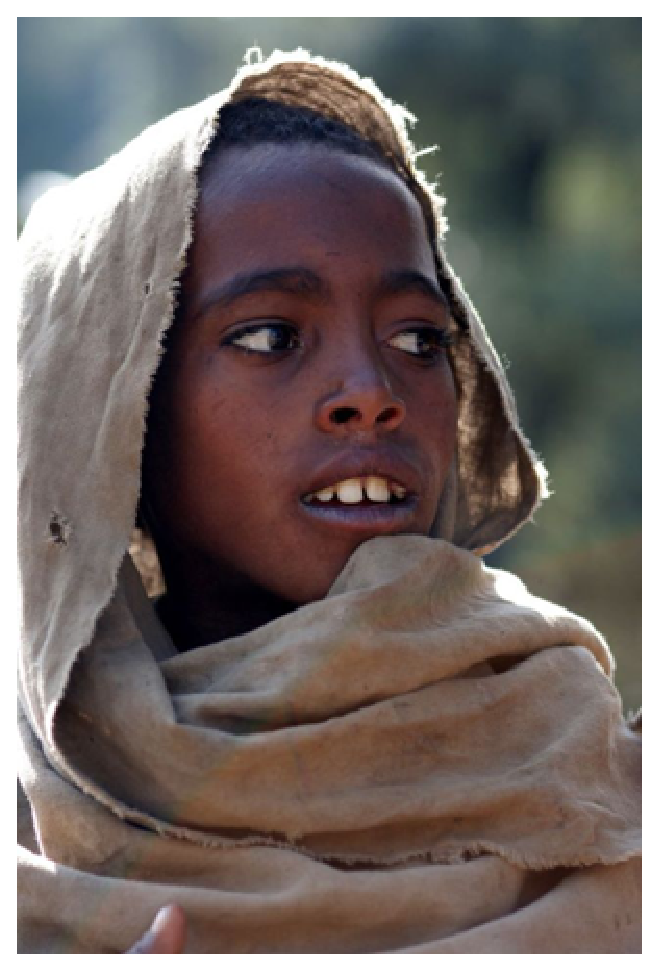
\includegraphics{img/etiopan.eps} \reflectbox{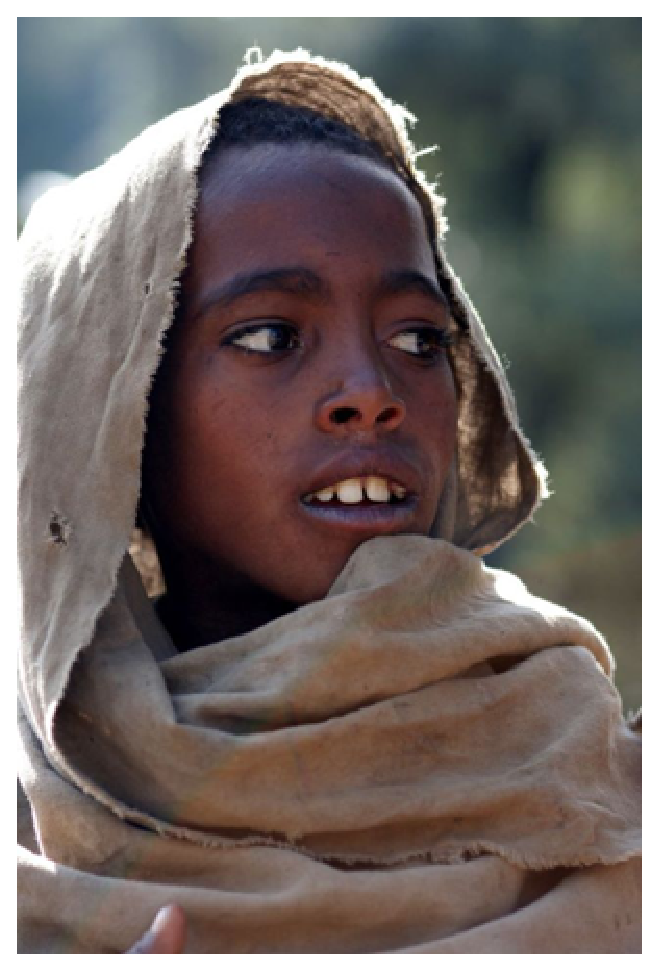
\includegraphics[]{img/etiopan.eps}}}
            \caption{Malý Etiopiánek a jeho bratříček}
            \label{img1}
        \end{figure}
        
    \newpage
    
    Rozdíl mezi vektorovým \dots
    \begin{figure}[h]
        \centering
        \scalebox{0.525}{
\includegraphics{img/oniisan.eps}}
        \caption{Vektorový obrázek}
        \label{img2}
    \end{figure}
    
    \dots a bitmapovým obrázkem
    
    \begin{figure}[h]
        \centering
        \scalebox{0.8}{
\includegraphics{img/oniisan2.eps}}
        \caption{Bitmapový obrázek}
        \label{img3}
    \end{figure}
    
    \noindent
    se projeví například při zvětšení.
    
    Odkazy (nejen ty) na obrázky \ref{img1}, \ref{img2} a \ref{img3}, na tabulky \ref{tab1} a \ref{tab2} a také na algoritmus \ref{alg1} jsou udělány pomocí křízových odkazů. Pak je ovšem potřeba zdrojová soubor přeložit dvakrát.
    
    Vektorové obrázky lze vytvořit i přímo v \LaTeX u, například pomocí prostředí \,\texttt{pciture}.
    
    \newpage
    \global\pdfpageattr\expandafter{\the\pdfpageattr/Rotate 90}
    
    %na vykresleni domecku vyuzit tento software: https://github.com/Headclass/Latex-Picture-Drawing-Tool/tree/main
    %slunce vykresleno manualne
    \begin{sidewaysfigure}[ht]
        \centering
        \setlength{\unitlength}{1mm}
        \begin{picture}(200, 100)
            \put(20, 80){\circle{20}}
            
            \put(32, 80){\line(1,0){5}}
            \put(8, 80){\line(-1,0){5}}
            
            \put(20, 92){\line(0,1){5}}
            \put(20, 68){\line(0,-1){5}}
            
            \put(28, 88){\line(1,1){4}}
            \put(28, 72){\line(1,-1){4}}
            
            \put(12, 88){\line(-1,1){4}}
            \put(12, 72){\line(-1,-1){4}}
            
            \qbezier(53, 95)(80, 95)(107, 95)
            \qbezier(107, 95)(112, 86)(117, 77)
            \qbezier(117, 77)(131, 77)(145, 77)
            \qbezier(145, 77)(154, 65)(163, 53)
            \qbezier(163, 53)(129, 53)(95, 53)
            \qbezier(95, 53)(93, 62)(91, 71)
            \qbezier(91, 71)(70, 71)(49, 71)
            \qbezier(49, 71)(51, 83)(53, 95)
            \qbezier(53, 37)(53, 54)(53, 71)
            \qbezier(53, 37)(72, 38)(91, 39)
            \qbezier(91, 39)(93, 36)(95, 33)
            \qbezier(159, 33)(156, 34)(153, 35)
            \qbezier(155, 53)(154, 44)(153, 35)
            \qbezier(159, 33)(127, 33)(95, 33)
            \qbezier(119, 53)(118, 43)(117, 33)
            \qbezier(127, 53)(126, 43)(125, 33)
            \qbezier(149, 53)(148, 43)(147, 33)
            \qbezier(147, 33)(145, 34)(143, 35)
            \qbezier(143, 35)(134, 35)(125, 35)
            \qbezier(143, 35)(144, 44)(145, 53)
            \qbezier(127, 41)(128, 41)(129, 41)
            \qbezier(111, 53)(111, 46)(111, 39)
            \qbezier(111, 39)(114, 36)(117, 33)
            \qbezier(97, 33)(97, 43)(97, 53)
            \qbezier(93, 37)(93, 48)(93, 59)
            \qbezier(91, 39)(101, 39)(111, 39)
            \qbezier(99, 39)(99, 46)(99, 53)
            \qbezier(107, 39)(107, 46)(107, 53)
            \qbezier(105, 45)(104, 45)(103, 45)
            \qbezier(69, 49)(72, 49)(75, 49)
            \qbezier(75, 49)(75, 53)(75, 57)
            \qbezier(75, 57)(72, 57)(69, 57)
            \qbezier(69, 57)(69, 53)(69, 49)
            \qbezier(85, 49)(85, 53)(85, 57)
            \qbezier(85, 57)(88, 57)(91, 57)
            \qbezier(91, 57)(91, 53)(91, 49)
            \qbezier(91, 49)(88, 49)(85, 49)
            \qbezier(107, 81)(107, 84)(107, 87)
            \qbezier(107, 87)(108, 87)(109, 87)
            \qbezier(109, 87)(109, 84)(109, 81)
            \qbezier(25, 1)(53, 3)(81, 5)
            \qbezier(91, 5)(116, 6)(141, 7)
            \qbezier(81, 5)(81, 13)(81, 21)
            \qbezier(81, 21)(85, 21)(89, 21)
            \qbezier(89, 21)(89, 13)(89, 5)
            \qbezier(89, 5)(90, 5)(91, 5)
            \qbezier(25, 1)(24, 10)(23, 19)
            \qbezier(23, 19)(25, 21)(27, 23)
            \qbezier(27, 23)(33, 25)(39, 27)
            \qbezier(39, 27)(44, 28)(49, 29)
            \qbezier(49, 29)(53, 29)(57, 29)
            \qbezier(57, 29)(63, 28)(69, 27)
            \qbezier(81, 25)(75, 26)(69, 27)
            \qbezier(81, 25)(85, 25)(89, 25)
            \qbezier(81, 25)(81, 23)(81, 21)
            \qbezier(89, 21)(89, 23)(89, 25)
            \qbezier(89, 25)(95, 27)(101, 29)
            \qbezier(101, 29)(106, 30)(111, 31)
            \qbezier(111, 31)(115, 31)(119, 31)
            \qbezier(119, 31)(125, 30)(131, 29)
            \qbezier(131, 29)(136, 28)(141, 27)
            \qbezier(141, 27)(145, 27)(149, 27)
            \qbezier(149, 27)(150, 26)(151, 25)
            \qbezier(151, 25)(147, 25)(143, 25)
            \qbezier(143, 25)(142, 26)(141, 27)
            \qbezier(141, 7)(142, 16)(143, 25)
            \qbezier(151, 25)(149, 13)(147, 1)
            \qbezier(147, 1)(86, 1)(25, 1)
            \qbezier(151, 23)(155, 24)(159, 25)
            \qbezier(159, 25)(160, 25)(161, 25)
            \qbezier(161, 25)(164, 24)(167, 23)
            \qbezier(167, 23)(173, 23)(179, 23)
            \qbezier(179, 23)(178, 24)(177, 25)
            \qbezier(177, 25)(181, 25)(185, 25)
            \qbezier(185, 25)(191, 23)(197, 21)
            \qbezier(197, 21)(192, 21)(187, 21)
            \qbezier(187, 21)(186, 21)(185, 21)
            \qbezier(185, 21)(178, 21)(171, 21)
            \qbezier(171, 21)(169, 22)(167, 23)
            \qbezier(169, 23)(167, 12)(165, 1)
            \qbezier(165, 1)(173, 1)(181, 1)
            \qbezier(181, 1)(182, 1)(183, 1)
            \qbezier(183, 1)(187, 1)(191, 1)
            \qbezier(191, 1)(194, 11)(197, 21)
            \qbezier(147, 1)(156, 1)(165, 1)
            \qbezier(29, 23)(29, 14)(29, 5)
            \qbezier(35, 25)(35, 15)(35, 5)
            \qbezier(41, 27)(41, 16)(41, 5)
            \qbezier(47, 29)(47, 17)(47, 5)
            \qbezier(53, 29)(53, 18)(53, 7)
            \qbezier(59, 29)(59, 17)(59, 5)
            \qbezier(65, 27)(65, 17)(65, 7)
            \qbezier(71, 25)(71, 16)(71, 7)
            \qbezier(77, 25)(77, 16)(77, 7)
            \qbezier(167, 37)(168, 42)(169, 47)
            \qbezier(169, 47)(173, 46)(177, 45)
            \qbezier(177, 45)(177, 47)(177, 49)
            \qbezier(177, 49)(178, 50)(179, 51)
            \qbezier(179, 51)(180, 52)(181, 53)
            \qbezier(181, 53)(182, 54)(183, 55)
            \qbezier(183, 55)(183, 56)(183, 57)
            \qbezier(183, 57)(182, 58)(181, 59)
            \qbezier(181, 59)(182, 60)(183, 61)
            \qbezier(183, 61)(183, 62)(183, 63)
            \qbezier(181, 63)(182, 63)(183, 63)
            \qbezier(181, 63)(180, 64)(179, 65)
            \qbezier(179, 65)(180, 66)(181, 67)
            \qbezier(181, 67)(179, 67)(177, 67)
            \qbezier(177, 67)(176, 67)(175, 67)
            \qbezier(175, 67)(176, 68)(177, 69)
            \qbezier(177, 69)(175, 70)(173, 71)
            \qbezier(173, 71)(173, 70)(173, 69)
            \qbezier(173, 69)(172, 70)(171, 71)
            \qbezier(171, 71)(170, 70)(169, 69)
            \qbezier(167, 69)(166, 69)(165, 69)
            \qbezier(165, 69)(164, 68)(163, 67)
            \qbezier(165, 63)(164, 63)(163, 63)
            \qbezier(161, 59)(162, 61)(163, 63)
            \qbezier(165, 63)(164, 65)(163, 67)
            \qbezier(167, 69)(168, 69)(169, 69)
            \qbezier(161, 59)(160, 58)(159, 57)
            \qbezier(161, 53)(160, 51)(159, 49)
            \qbezier(159, 49)(160, 48)(161, 47)
            \qbezier(161, 47)(162, 46)(163, 45)
            \qbezier(163, 45)(165, 46)(167, 47)
            \qbezier(167, 47)(168, 47)(169, 47)
            \qbezier(169, 37)(169, 42)(169, 47)
            \qbezier(95, 27)(95, 18)(95, 9)
            \qbezier(101, 29)(101, 19)(101, 9)
            \qbezier(107, 31)(107, 20)(107, 9)
            \qbezier(113, 31)(113, 20)(113, 9)
            \qbezier(119, 31)(119, 20)(119, 9)
            \qbezier(125, 31)(125, 20)(125, 9)
            \qbezier(131, 29)(131, 19)(131, 9)
            \qbezier(137, 27)(137, 19)(137, 11)
            \qbezier(153, 23)(152, 13)(151, 3)
            \qbezier(157, 25)(156, 14)(155, 3)
            \qbezier(161, 25)(160, 15)(159, 5)
            \qbezier(165, 23)(163, 13)(161, 3)
            \qbezier(159, 5)(159, 4)(159, 3)
            \qbezier(165, 11)(166, 11)(167, 11)
            \qbezier(25, 1)(21, 1)(17, 1)
            \qbezier(17, 1)(16, 10)(15, 19)
            \qbezier(15, 19)(16, 21)(17, 23)
            \qbezier(25, 21)(24, 20)(23, 19)
            \qbezier(17, 23)(21, 23)(25, 23)
            \qbezier(25, 23)(24, 21)(23, 19)
            \qbezier(23, 19)(19, 19)(15, 19)
            \qbezier(3, 27)(18, 36)(33, 45)
            \qbezier(33, 45)(37, 47)(41, 49)
            \qbezier(41, 49)(47, 50)(53, 51)
            \qbezier(155, 43)(161, 41)(167, 39)
            \qbezier(167, 39)(176, 37)(185, 35)
            \qbezier(185, 35)(192, 32)(199, 29)
            \qbezier(105, 33)(106, 32)(107, 31)
            \qbezier(117, 33)(118, 32)(119, 31)
            \qbezier(125, 33)(131, 30)(137, 27)
            \qbezier(157, 33)(168, 29)(179, 25)
            \qbezier(25, 5)(53, 7)(81, 9)
            \qbezier(89, 9)(115, 10)(141, 11)
            \qbezier(151, 3)(151, 2)(151, 1)
            \qbezier(155, 3)(155, 2)(155, 1)
            \qbezier(159, 3)(159, 2)(159, 1)
            \qbezier(161, 3)(161, 2)(161, 1)
            \qbezier(15, 21)(9, 23)(3, 25)
            \qbezier(3, 25)(3, 26)(3, 27)
            \qbezier(3, 25)(4, 15)(5, 5)
            \qbezier(9, 23)(10, 14)(11, 5)
            \qbezier(17, 5)(11, 5)(5, 5)
            \qbezier(17, 1)(10, 1)(3, 1)
            \qbezier(3, 1)(3, 14)(3, 27)
            \qbezier(199, 29)(199, 28)(199, 27)
            \qbezier(199, 27)(194, 25)(189, 23)
            \qbezier(199, 27)(197, 16)(195, 5)
            \qbezier(195, 25)(195, 23)(195, 21)
            \qbezier(195, 5)(194, 5)(193, 5)
            \qbezier(53, 43)(51, 40)(49, 37)
            \qbezier(49, 37)(51, 37)(53, 37)
            \qbezier(53, 43)(47, 43)(41, 43)
            \qbezier(41, 43)(45, 47)(49, 51)
        \end{picture}
        \caption{Přední strana našeho domu}
        \label{img4}
    \end{sidewaysfigure}
\end{document}